\providecommand{\main}{..}
\documentclass[\main/master.tex]{subfiles}
\begin{document}
\newspacing
\chapter{Methods and results}\label{chapter:Methods and results}

\section{System structure}
\subsection{Experiment setup}
\begin{figure}[htbp]
	\centering
	\fbox{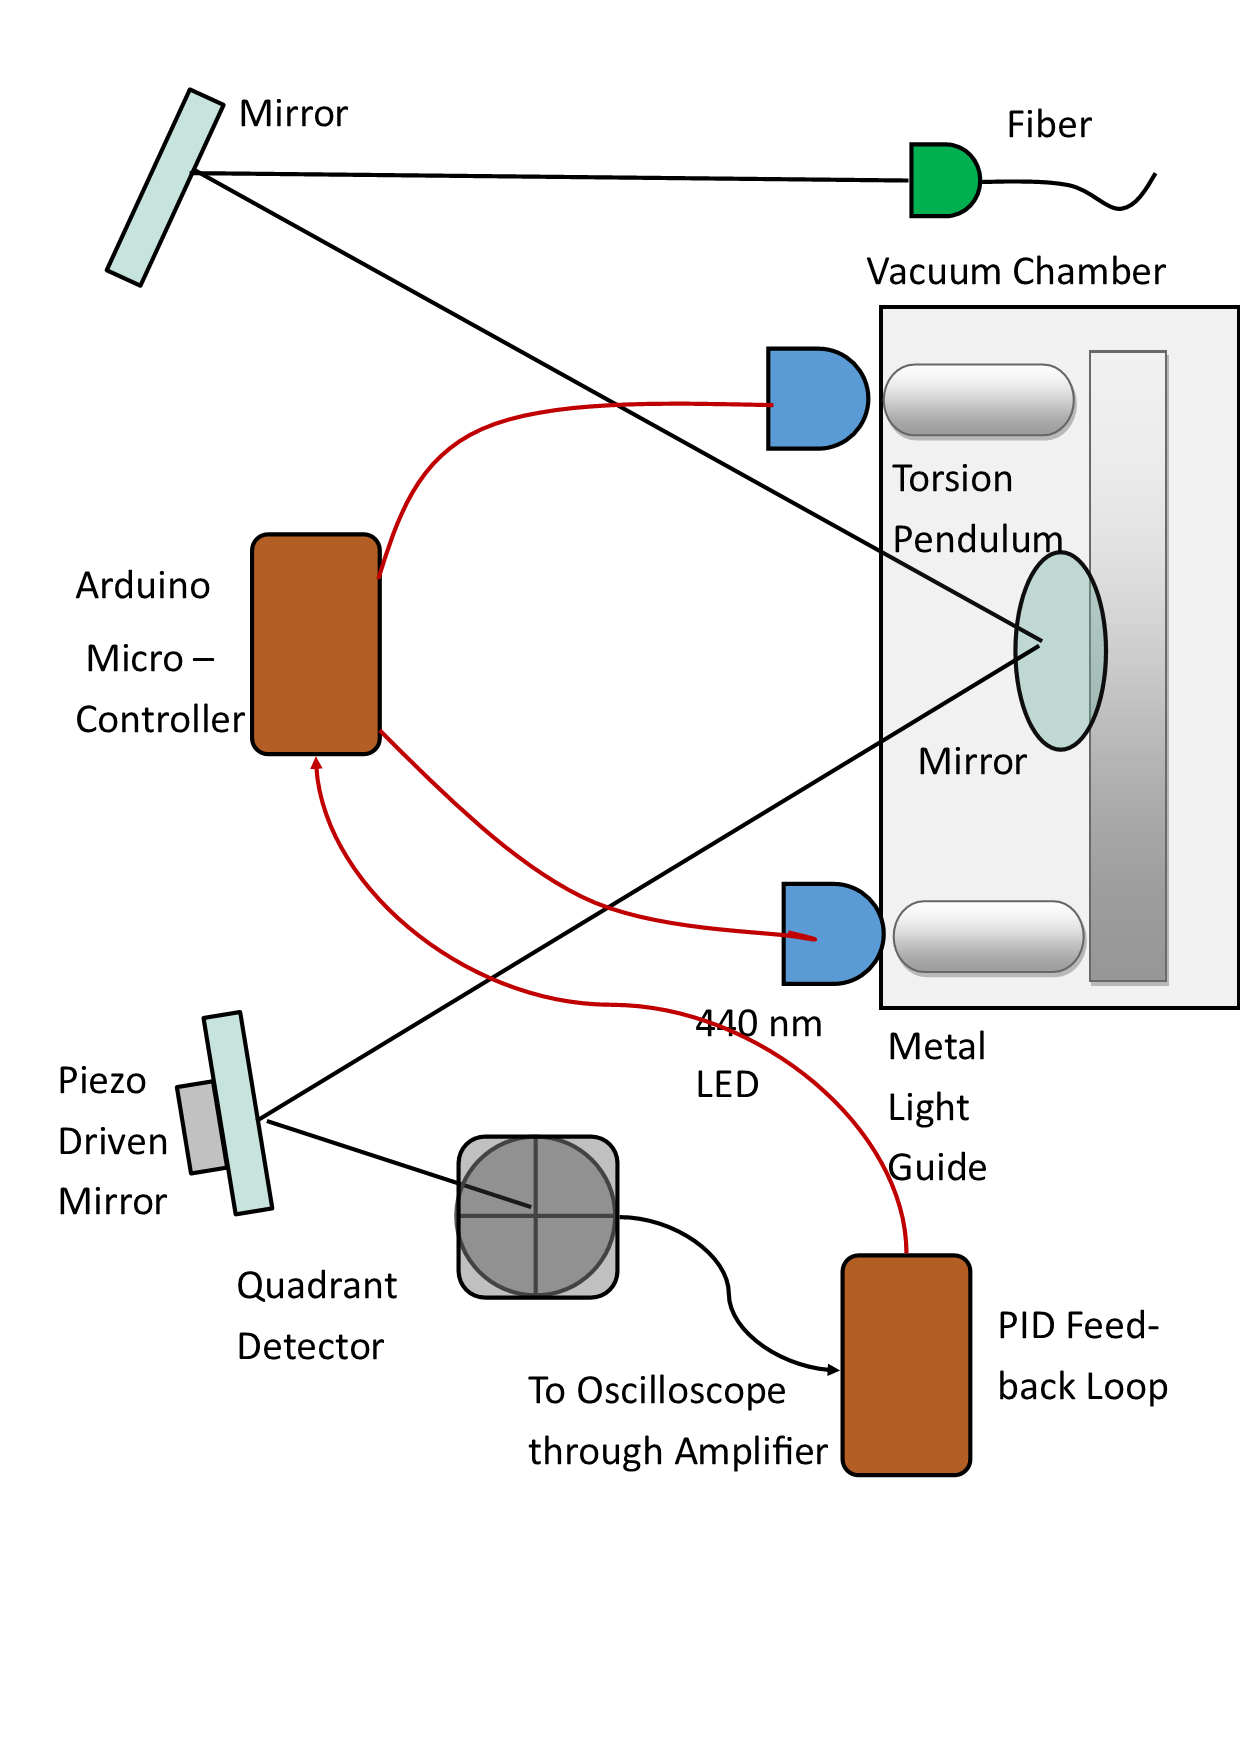
\includegraphics[scale=0.2]{\main/images/4 - methods and results/setup.png}}
	\caption[The experiment setup]{The experiment setup}
	\label{fig:setup}
\end{figure}
\FloatBarrier
\par\noindent
The experiment setup, shown in fig.~\ref{fig:setup}, is composed of a torsion pendulum placed inside a vacuum chamber, a tilt angle measurement system and a feedback system. The experiment setup is placed inside an acoustic box, which is not shown in the figure. The angle is measured by a laser beam deflected by the pendulum's front mirror and detected by a quadrant detector. The detector is connected to a computer by an oscilloscope through a signal amplifier. The light reflected from the pendulum mirror is reflected by a piezo driven mirror, which is tuned so that the reflected light would strike the detector's center (the PID needs a reference for error calculations). 
\par\noindent
The feedback system is composed of two LED light sources, modulated in real time by an Arduino micro-controller which is controlled by the PID feed-back loop in the computer. The LED light sources are each coupled to a side mass of the pendulum. The light is passed through the vacuum chamber by having transparent windows (viewports) on the sides of the chamber. 
\par\noindent
The vacuum chamber is connected to a vacuum engine, which is pumping out gas and lowering the pressure. When the desired pressure is achieved, the vacuum engine is disconnected using the valve and turned off, and the acoustic box is sealed. When the oscillations settle down to a level which could be affected by the weak torques caused by radiation pressure, the angle is read in real time by the PID algorithm, and radiation-pressure torque is exerted by the LED's flux for damping down the pendulum noises.
\subsubsection{Design of the system}
\begin{figure}[htbp]
	\centering
	\fbox{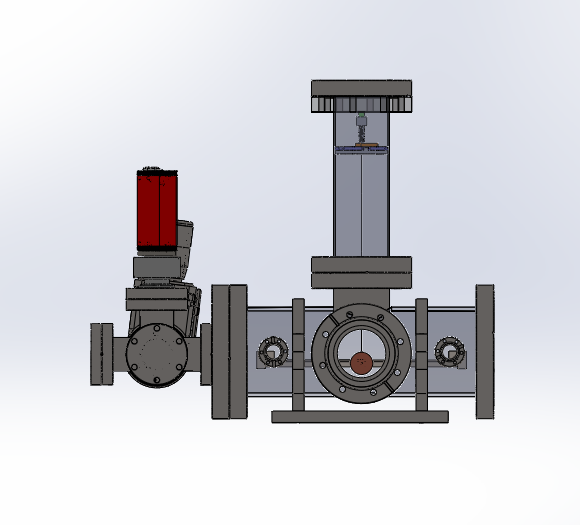
\includegraphics[scale=0.5]{\main/images/4 - methods and results/total_chamber.png}}
	\caption[Total chamber]{The system structure}
	\label{fig:Total chamber}
\end{figure}
\FloatBarrier
\par\noindent
The design of torsional pendulum and vacuum chamber, shown in fig.~\ref{fig:Total chamber}, was carried out using the software Solid Works. The torsional pendulum was manufactured by the university workshop, and the vacuum chamber was manufactured at HTC Vacuum. The assembling was performed at the HUJI lab. The system had undergone changes, and the final design of the system is presented. 
\par\noindent
As shown previously (eq.~\ref{eqn:drag force2}, eq.~\ref{eqn:total Brownian energy}, eq.~\ref{eqn:heat conduction}, eq.~\ref{eqn:acoustic power}), friction, Brownian motion energy, thermal power and acoustic waves are pressure dependent and are considerably reduced by maintaining low pressure. Therefore, the torsional pendulum is placed inside a vacuum chamber. Magnetic noise is reduced by choosing low magnetic permeability materials, avoiding capacitance and using a Faraday cage. 
\par\noindent
The vacuum chamber is placed inside an acoustic box, further reducing acoustic waves and magnetic noise. In order to maintain low pressure for long periods, the system is designed to minimize the outgassing rate by both, choosing low outgassing materials and avoiding air pockets inside the devices. 
\subsection{Vacuum chamber design}
\begin{figure}[htbp]
	\centering
	\fbox{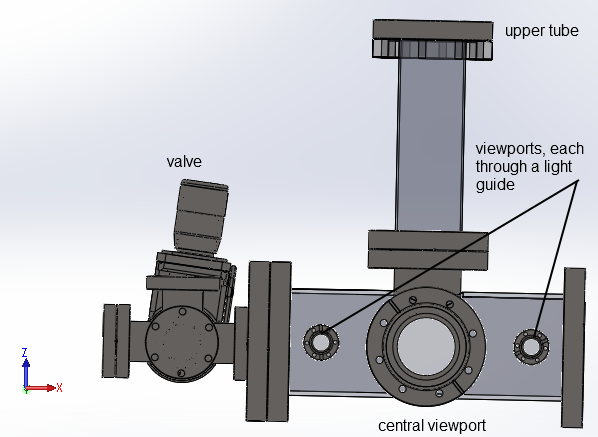
\includegraphics[scale=0.5]{\main/images/4 - methods and results/chamber_front_names.png}}
	\caption[Vacuum chamber, front view]{Vacuum chamber, front view}
	\label{fig:chamber front}
\end{figure}
\FloatBarrier

\par\noindent
The vacuum chamber, shown in fig.~\ref{fig:chamber front}, is composed of two cylindrical tubes placed one over the other with three view ports in front and light guides. The chamber is connected to a vacuum engine and gauge. The vacuum engine is connected to the chamber through a valve. The measurements are conducted when the valve is closed and the engine is off, to prevent rotation noise.

\subsubsection{Chamber viewports}
\par\noindent
The lower tube has three viewports. The central viewport is located in front of the pendulum's front mirror. The central viewport has a $68.3 [mm]$ view diameter where the mirror is located $82 [mm]$ away, giving a measurement FOV of about $39^0$ degrees. The other two small viewports are located in front of the pendulum's side masses and they are used for damping down the pendulum noises. They are connected to the chamber through light guides. The view ports are transparent for light in the $550-1100 [nm]$ range, with about 98$\%$ power transmittance in this range. 


\subsubsection{Vacuum maintenance}
\par\noindent
Due to the measurement sensitivity, the vacuum engine pumping must be off during measurement. Accordingly, the main limitations to the maintenance of low pressure are the leakage $Q_L$ from the outside (eq.~\ref{eqn:leak rate}) and the outgassing $Q_{des}$ inside the chamber (eq.~\ref{eqn:desorption rate}), thus increasing of the pressure at a constant rate over time. Due to the pendulum's shape and size, the vacuum chamber has large volume (high leak rate) and large surface area (high outgassing rate). 
\par\noindent
In order to minimize the pressure increase rate, the vacuum chamber is built using CF components which are designed for ultra high vacuum, and minimize the leak rate. Also, to reduce outgassing, the torsional pendulum and vacuum chamber were baked-out at $120 C^0$ for a week, using resistive wire. 
\par\noindent
The chamber volume is $V = 4.75\cdot 10^{-4}[m^3]$, and the measured pressure at the experiments after cooling down is $P \approx 1\cdot 10^{−2} [pa]$ for a month without pumping with the vacuum engine.
\subsection{Torsional pendulum design}
 
\begin{figure}[htbp]
	\centering
	\fbox{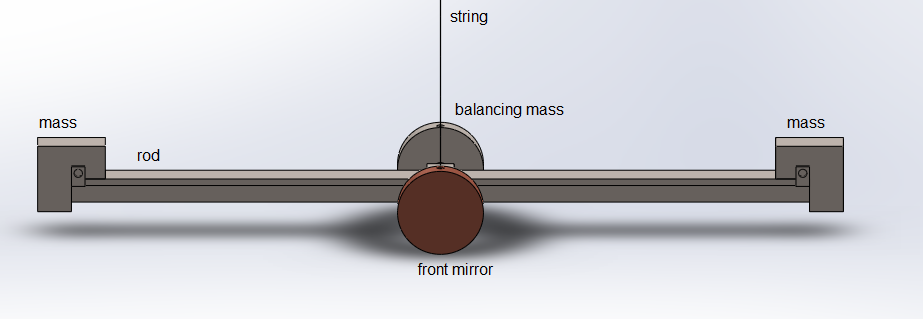
\includegraphics[scale=0.3]{\main/images/4 - methods and results/pendulum_front_names.png}}
	\caption[Torsional pendulum, front view]{Torsional pendulum, front view}
	\label{fig:pendulum front}
\end{figure}
\FloatBarrier
\par\noindent
The torsional pendulum design, shown in fig.~\ref{fig:pendulum front}, is composed of a thin rod with the length $2l$, string with the length $h$, two identical masses $m$ on the sides, a front mirror and a balancing mass to balance the center of mass. 
\begin{figure}[htbp]
	\centering
	\fbox{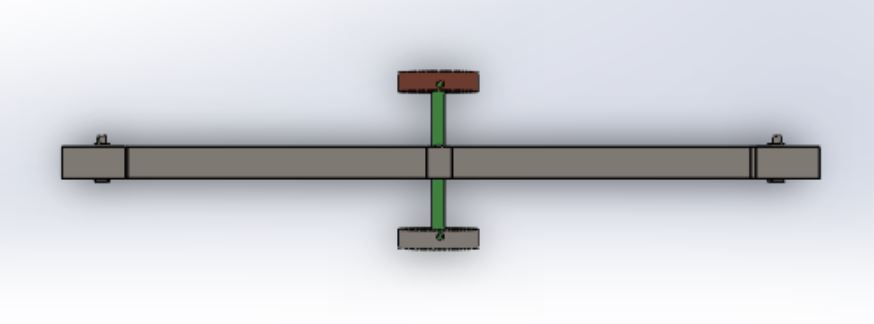
\includegraphics[scale=1.2]{\main/images/4 - methods and results/pendulum_top.JPG}}
	\caption[The torsional pendulum, top view]{The torsional pendulum, top view}
	\label{fig:pendulum top}
\end{figure}
\FloatBarrier 
\par\noindent
The center of mass is balanced using a balancing mass with similar shape and weight as the mirror on the other side, as shown in fig.~\ref{fig:pendulum top}. The balancing mass and the mirror are connected from their centers to the pendulum by a beam with length $w$, thus the overall downward torque $\tau_z$ with tilt angle $\phi$ is given by:
\begin{equation}
\tau_z = r_1\cdot m_1 g \cdot cos\phi - r_2\cdot m_2 g \cdot cos \phi\ = g\cdot cos\phi( m_1 r_1  - m_2 (w-r_1) )    \label{eqn:downward torque}
\end{equation}
Where $m_1$, $m_2$ are the masses of the mirror and the balancing mass, and $r_1$, $r_2$ are their distance from the pendulum's center of mass respectively. The beam allows to cancel out the torque $\tau_z$ by accurate adjustment of the distance $r_1$, given by: 
\begin{equation}
 r_1 = \frac{w}{\frac{m_1}{m_2}+1}  \label{eqn:downward torque cancelled}
\end{equation}
\subsubsection{Adjustable mount}
\begin{figure}[htbp]
	\centering
	\fbox{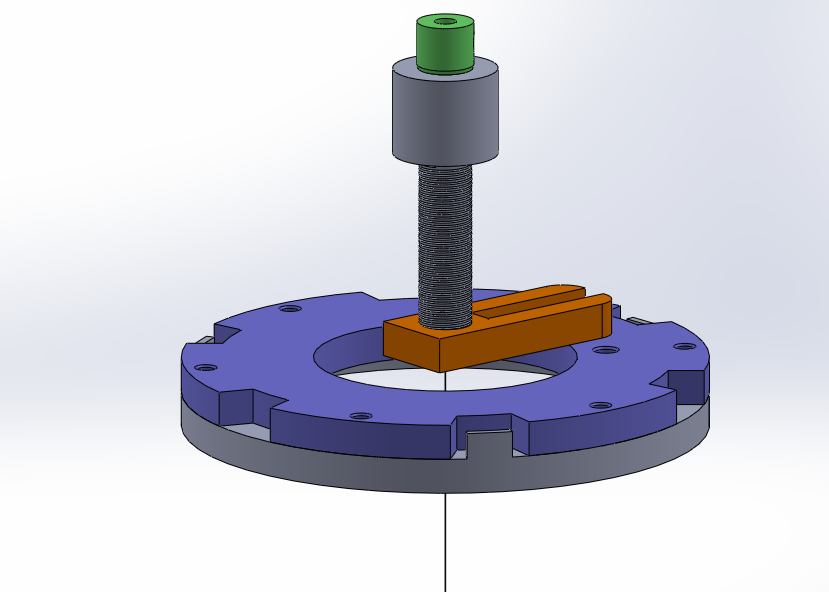
\includegraphics[scale=0.2]{\main/images/4 - methods and results/mount.png}}
	\caption[The pendulum mount]{The pendulum mount}
	\label{fig:mount}
\end{figure}

\par\noindent
The adjustable mount, shown in fig.~\ref{fig:Total chamber}, is used for adjusting the height, distance and angle of the torsional pendulum. The torsional pendulum string is held by the adjustable mount from the upper tube of the vacuum, placing it accurately in front of the viewports. 

\subsubsection{Design constraints}
\par\noindent
The chosen pendulum dimensions are designed to achieve large angle sensitivity to the torque caused by a the gravity field (small string torsion coefficient $\kappa$ is needed, see eq.~\ref{eqn:theta average}) while maintaining large angle sensitivity to the measured mass (longer oscillation time period $T$, see eq.~\ref{eqn:theta average}). For a torsional pendulum with moment of inertia $I$ and string torsion coefficient $\kappa$, the oscillation time period $T$ is given by (eq.~\ref{eqn:undamped_omega}): 
\begin{equation}
T = 2\pi\sqrt{\frac{I}{\kappa}}  =  2\pi\sqrt{\frac{I}{\frac{G}{h} \frac{\pi d^4}{32}}}  \label{eqn:undamped_motion_equation_4}
\end{equation}
\par\noindent
According to eq.~\ref{eqn:undamped_motion_equation_4}, longer string length $h$ with smaller diameter $d$ results in small string torsion coefficient while having a large period time.
\par\noindent
The string is made of tungsten that is both, vacuum compatible (material with low outgassing) and has high tensile strength \cite{tungsten}, and is holding the pendulum robustly inside the vacuum chamber while having small string diameter. 
\par\noindent
In order to minimize the magnetic noise in the measurements, the torsional pendulum is made out of stainless steel 316 (instead of stainless steel 304) which has lower magnetic permeability \cite{SS316}, and the chosen front mirror is made fully of oxygen-free copper (OFC) instead of coated glass thus preventing capacitance. 
\subsubsection{Technical information}
The designed elements specifications are:
\begin{multicols}{2}
\raggedcolumns
\begin{easylist}
& Torsional beam;
&& Stainless steel 316.
&& length $2l=0.218 [m]$.
&& cross section $A =1.14\cdot10^{-2}[m^2]$.
&& mass weight $20.5\cdot10^{-3} [kg]$.
&& total weight $m_1=150\cdot10^{-3} [kg]$.
%& Mirror;
%&& OFC, gold coated.
%&& diameter of 1 inch.
\end{easylist}
\columnbreak
\begin{easylist}
& Tungsten string;
&& 99.95\% pure Tungsten
&& shear modulus $G = 130-160 [Gpa]$.
&& length $h= 0.249 [m]$.
&& diameter $d=80\cdot10^{-6}[m]$.
\end{easylist}
\end{multicols}
\subsection{Torsional motion}
Friction (eq.~\ref{eqn:drag force2}), Brownian motion (eq.~\ref{eqn:total Brownian energy}), thermal flow (eq.~\ref{eqn:heat conduction}) and acoustic waves (eq.~\ref{eqn:acoustic power}) are pressure dependent, and are reduced by having a lower pressure. The measurement system is placed inside an acoustic box, further reducing the acoustic power and also reducing magnetic noise as a Faraday cage (eq.~\ref{eqn:skin depth}). 
\par\noindent
The acoustic box is a Faraday cage with 76 mm thickness, blocking magnetic fields with frequencies $f \ge 30 [Hz]$ from the environment. The vacuum chamber is a second cage that further blocks magnetic noise from the electronic system placed inside the acoustic box. The vacuum chambers is made out of approximately 3 mm thick stainless steel, blocking magnetic fields with frequencies $f\ge 20 [KHz]$ and reducing magnetic noise with lower frequencies.
\par\noindent
Initially the pendulum a driven oscillator (eq.~\ref{eqn:driven_motion_equation_2}) driven by small torques, consisted of black body radiation and the pressure dependent noises. Gradually the pressure dependent friction is damping the velosity, until the pendulum reaches an amplitude at which the friction is equal to the driving noises. The equilibrium amplitude is independent of the initial amplitude, but rather the pressure and temperature. Due to the low pressure the damping of the friction is very slow. After 8 hours of damping, the torsional pendulum reaches equilibrium with a measured amplitude of $\theta_{max}^{eq}\approx 1\cdot10^{-5}[rad]$ (the same result is achieved also after a week). From the long damping time it can be shown that the friction coefficient is very small, allowing to neglect the friction at small amplitudes.
\par\noindent
Except for the torsional mode (in which we are interested) there is also a bouncing mode with a period of $T_b\approx 2\pi\sqrt{\frac{h}{g}}\approx 1[s]$. The bouncing mode is masking the measurement, and filtered out in real time. 
As shown in eq.~\ref{eqn:Brownian uncertainty 3}, without noises the fundamental quantum uncertainty at room temperature results with an amplitude of  $\theta_{max}  \approx 4\cdot 10^{-8} [rad] $, meaning the pendulum noises  
\par\noindent
 
\par\noindent
\subsection{results}
The system measured results compared to the expected results from the equations are given by:
\begin{multicols}{2}
\raggedcolumns
\begin{easylist}
& expected;
&& $I = 0.487\cdot10^{-3}[kg\cdot m^2]$
&& $\kappa = 2.1\cdot10^{-6}[\frac{N\cdot m}{rad}] - 2.6\cdot10^{-6} [\frac{N\cdot m}{rad}]$
&& $T = 96[s] - 86 [s]$
\end{easylist}
\columnbreak
\begin{easylist}
& measured;
&& $\kappa = 2.7\cdot10^{-6}[\frac{N\cdot m}{rad}]$
&& $T = 84[s]$
&& $\theta_{max}^{eq} \approx 1\cdot10^{-5}[rad]$
\end{easylist}
\end{multicols}
The expected $\kappa$, $T$ have a range due to uncertainty of the string tensile strength $G$. The equilibrium amplitude $\theta_{max}^{eq}$ is an experimental value, depended on the amount of noise actually reduced, thus do not have an expected simulated value.



\section{Proportional–Integral–Derivative (PID) controller}
\subsection{Control stability}
The PID feed-back loop is continuously calculating the error value of the measured signal from a defined set point, which is the deviation of the pendulum amplitude from a $SP$ angle $e(t) =SP -\theta(t) $. The PID aims to reach the $SP$ with critical damping of the process (the torsional pendulum) by damping the error to zero. 
\par\noindent
In control theory there are two wanted conflicting properties; an accurate response (small overshoot), and small risetime (fast response). A PID control does not guarantee optimal control or stability of the process. When PID not tuned correctly, it can either overshoot or have a slow response, both resulting with a driven oscillator. The PID response to error (shown in eq.~\ref{eqn:PID response}) defines how much will the oscillator overshoot the $SP$.
\par\noindent
Overshoot is when the value of output signal (the actual response) exceeds the target value (the wanted response), thus the response is not accurate. The overshoot of a second order system is given by:
\begin{equation}
overshoot =  \frac{output-target}{target} = e ^{\frac{-\xi\pi}{\sqrt{1-\xi^2}}}  \label{eqn:overshoot}
\end{equation}
\par\noindent
Where $\xi$ is the damping ratio of the oscillator defined in eq.~\ref{eqn:system damping ratio}. As seen in eq.~\ref{eqn:overshoot} when the PID gains are too high, instead of critical damping there is overdamping, which is causing overshoot. Due to the high gains the overshoot response overshoots again to the other side, causing the system to be an unwanted driven oscillator (shown in eq.~\ref{eqn:driven_motion_equation_2}). A slow response causes phase delay between the signal and the equivalent PID response, resulting again with a driven oscillator.
\subsection{Damped oscillator}
The torsional pendulum is a simple harmonic oscillator with oscillations amplitude $\theta_{max}$ and velocity given by $\dot{\theta}(t) =\frac{2\pi}{T} \theta_{max}( t)$ (see eq.~\ref{eqn:undamped_motion_equation_solved}). The PID mainly acts as friction, gradually slowing the oscillations velocity, with a torque $\tau_{PID}$ given by:
\begin{equation}
\tau_{PID}(t) = -\gamma\dot{e}(t) =  -\gamma\cdot [\dot{SP} -\dot{\theta}(t)] =-\gamma\cdot [0-\dot{\theta}(t)]  =  \gamma\dot{\theta}(t) =  \gamma\frac{2\pi}{T} \theta_{max}( t) 
\label{eqn:friction_torque_pid}
\end{equation}
\par\noindent
Accordingly, the PID damping coefficient $\gamma$ is given by (eq.~\ref{eqn:damped_motion_equation}):
\begin{equation}
\gamma  =  \frac{\tau_{PID}(t)}{\frac{2\pi}{T} \theta_{max}( t) } =\frac{\tau_{max}}{\theta_{max}}\cdot \frac{ T}{2\pi}          \label{eqn:pid damping coefficient}
\end{equation}
Where $\tau_{max}$ is the maximal torque exerted by the PID. When damping using the PID the damping type, defined by the damping ratio $\xi$, and the damping time $\tau$ are given by (eq.~\ref{eqn:damping_time}):
\begin{equation}
\xi = \frac{T}{2 \pi \tau } =  \frac{T}{2 \pi  }\frac{\gamma}{2I}  = \frac{ \tau_{max}}{\theta_{max}} \cdot \frac{T^2}{8\pi^2 I}  \label{eqn:damping_time_pid}
\end{equation}
The PID damping $\gamma$, the damping time $\tau$ and the damping type depend on the ratio $\theta_{max}/\tau_{max}$. When torque is too small compared to the amplitude, the damping affect is negligible, resulting with a highly underdamped oscillator with infinite damping time. The PID must be able to exert torques which can critically damp the equilibrium amplitude (eq.~\ref{eqn:critically_damped_motion_equation}), the PID maximal torque $\tau_{max} $ is given by:
\begin{equation}
\tau_{max} (\xi = 1)\geq\frac{ 8 \pi^2 I }{T^2}\cdot\theta_{max}^{eq} = \frac{  8 \pi^2 \cdot 0.487\cdot10^{-3} }{(84)^2}\cdot 1\cdot10^{-5} = 5.45\cdot10^{-11}[N\cdot m]
\label{eqn:damping_torque_pid}
\end{equation}
\par\noindent
Since, the torque is proportional to the oscillations velocity (eq.~\ref{eqn:friction_torque_pid}), it needs a high modulation frequency compare to the oscillations frequency (to prevent phase delay), and high modulation range compare to the amplitude (to avoid overshoot). 
\subsection{Radiation-pressure torque}
The PID torque was chosen to be a Radiation-pressure torque. The setup is composed of two light sources in front of the two torsional pendulum sides, each with flux modulated in time differently $\Theta_i(t)$. As seen in eq.~\ref{eqn:net_gravitation_torque}, the difference between two torques adds an external net torque. Assuming both light fields are very close to be perpendicular to the surface with negligible incidence angles $\alpha_1\approx\alpha_2\approx 0$ and have the same coupling efficiency $\eta$, using eq.~\ref{eqn:radiation_force_power}, the radiation-pressure net torque $\tau(t)$ is:  
\begin{equation}
\tau(t) = l\cdot F_1(t) \cdot cos\alpha_1 - l\cdot F_2(t) \cdot cos\alpha_2\approx l(F_1(t) - F_2(t)) \approx \frac{2l\eta}{{c}} \Delta \Theta(t) \label{eqn:radiation torque}
\end{equation}
The radiation-pressure net torque is controlled by changing the difference between the light sources' flux $\Delta \Theta(t)$. The maximal tourqe $\tau_{max}$ (eq.~\ref{eqn:damping_torque_pid}) is at the maximal difference $\pm \Theta_{max}$. Thus, the needed flux for critical damping with optical setup efficiency $\eta$ is given by: 
\begin{equation}
\eta\Theta_{max} \geq \frac{\tau_{max}}{\frac{2 l}{c}}\approx \frac{5.45\cdot10^{-11}}{\frac{ 0.218}{3\cdot10^{8}}}\approx 75 [mW]
\label{eqn:max radiation torque}
\end{equation}

\subsection{Laser setup}
Initially the modulated light sources were composed of a single laser diode coupled in series into two acousto optic modulators (AOM), with special filtered mode using optical fibers. The AOMs divides the single coherent light beam into two beams, with the intensity ratio modulated, resulting with controlled modulation of the light sources difference.
\par\noindent
The apparatus had dynamic range of $10000$ steps and modulation  frequency of $1 [Hz]$. The setup minimized uncertainties of the light intensity since both light sources had a mutual source, partly cancelling internal noises such as thermal and shot noise. 
\par\noindent
The apparatus uncertainty due to the non linearity of the AOM response and laser power fluctuations proved to be larger than the uncertainties of the intensity difference. Also, modulation frequency proved to be more important than modulation range. Due to the conclusions, the PID torque was changed to two controlled light emitting diode (LED) sources.
\subsection{Light emitting diode (LED)}
The light emitting diode (LED) is a semiconductor light source with high power and long lifetime. A forward voltage applied to a p-n junction, causes electron injection which recombine with holes. The recombination releases energy in form of spontaneous emission photons (incoherent light). Due to the electrons life time, the LED could be modulated up to $100MHz$. The LED forward voltage is given by the Shockley diode equation for p-n junctions, $V_l \approx n V_T ln10 log_{10} (\frac{I_l}{I_s})$. Where $I_l$ is the LED current, $I_s$ is the saturation current, $n$ is the emission coefficient, and $V_T$ is the thermal voltage. 
\par\noindent
Since $V_l$ varies as the logarithm of the current, it is approximately constant over wide current range. In the driving circuit a resistor $R$ is connected in series with the LED to stabilizes the current. The LED light flux with circuit of $N$ voltages supplies $V$ in parallel is given by:
\begin{equation}
\Theta = I_l\cdot V_l  =\frac{N\cdot V-V_l}{R}\cdot V_l\approx \frac{N\cdot V_l\cdot V}{R}\label{eqn:led power}
\end{equation}
\par\noindent
The LED illumination angle varies between $45^0-120^0$. Since emitted light is incoherent it is hard to focus it to a point (not diffraction limited). In order to overcome the large illumination angle, the LED light sources are coupled to light guides (the vacuum chamber viewports were designed to have light guides in front). A light guide is a pipe made of thin filaments causing internal reflections, designed to illuminate small areas, regardless of the spectral characteristics of the light source. The light guide efficiency $\eta$ is mainly dependent on the cross section and length of the lightguide. 

\subsection{Arduino microcontroller}
\begin{figure}[htbp]
	\centering
	\fbox{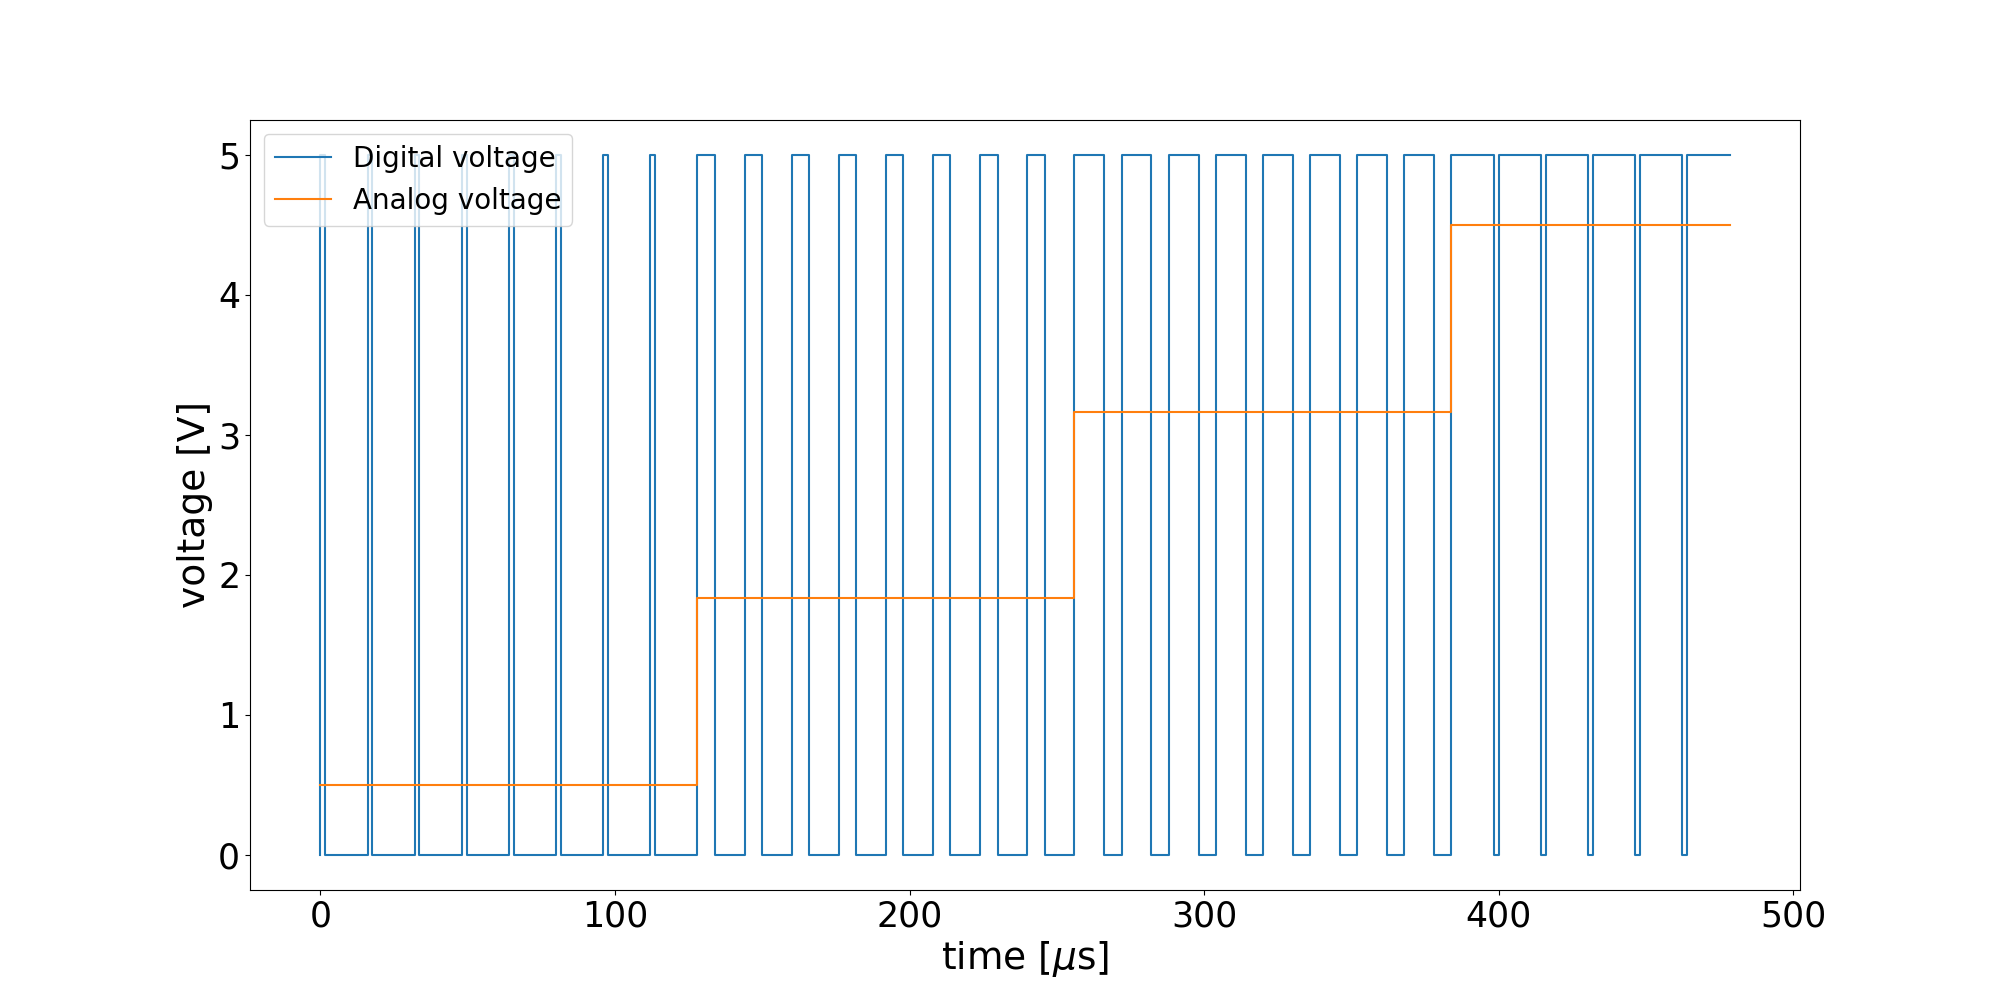
\includegraphics[scale=0.11]{\main/images/4 - methods and results/duty_cycle.png}}
	\caption[The PWM analog voltage]{The PWM analog voltage}
	\label{fig:duty_cycle}
\end{figure}
\FloatBarrier
\par\noindent
The Arduino Mega 2560 is an inexpensive 8-bit microcontroller with $16 [MHz]$ clock and multiple Pulse Width Modulation (PWM) analog outputs, which are using a digital output of $V_d = 5[V]$. As shown in fig.~\ref{fig:duty_cycle}, the controller switches the output signal on and off, generating a square wave with period $T$. Pulse width ($PW$) is the time duration in which the signal is on, the controller is able to modulate the $PW$, and thus change the duty cycle which is the ratio of time signal is on compared to off $D(t) = \frac{PW(t)}{T}\cdot 100$. The PWM is proportional to the analog average voltage $V_a$ given by: 
\begin{equation}
V_a(t) = \frac{ PW(t)\cdot V_d}{ T}  = \frac{V_d}{100}\cdot D(t)   \label{eqn:pwm voltage}
\end{equation}
Since the Arduino clock is connected to all PWM pins, they are all synchronized and have the same voltage, frequency and phase, allowing to connect them in parallel. The clock must have at least 120 periods of square waves before it can change to a new duty cycle value, this limits the voltage modulation frequency. Another limitation to the duty cycle change rate is the controller bit-rate. Accordingly, PWM maximal frequency is given by:
\begin{equation}
f_{PWM} = \frac{1 }{120T}= \frac{1 }{120 \frac{8-bit }{16MHz}}  \approx 500[Hz]	    \label{eqn:pwm frequency}
\end{equation}

\subsection{LED circuit}
The LED circuits are each composed of a blue LED with $V_l\approx 4.5V$, with $N=6$ parallel PWM pins for the supply voltage (eq.~\ref{eqn:pwm voltage}) and resistor $R = 200\Omega$. Due to coupling efficiency and size difference between the output beam from the lightguide and the pendulum sides, the efficiency of flux hitting the pendulum is estimated $\eta = 0.7$, thus with LED flux given by eq.~\ref{eqn:led power}, the PID torque $\tau_{PID}(t)$ is given by (eq.~\ref{eqn:radiation torque}):
\begin{equation}
\tau_{PID}(t) \approx \frac{2l\eta}{{c}} (\Theta_1(t) -\Theta_2(t)) \approx \frac{2l\eta}{{c}} \cdot\frac{N V_l V_d}{100R}(D_1(t) -D_2(t))  \approx   3.4\cdot 10^{-12}(D_1(t) -D_2(t)) 
\label{eqn:led torque}
\end{equation}
\par\noindent
The torque is controlled by the duty cycle $D(t)$ varying between $0-100$ with 8bit resolution, thus generating torques up to $\tau = \pm 3.4\cdot10^-{10} [N\cdot m]$ with modulation steps of $\Delta\tau = 1.34\cdot10^-{12} [N\cdot m]$ and modulation frequency up to $500[Hz]$ (see eq.~\ref{eqn:pwm frequency}). The LED light source has approximately a linear response which minimizing the overshoot, and a fast response minimizing the phase delay.

\section{Results} 
\begin{figure}[htbp]
	\centering
	\fbox{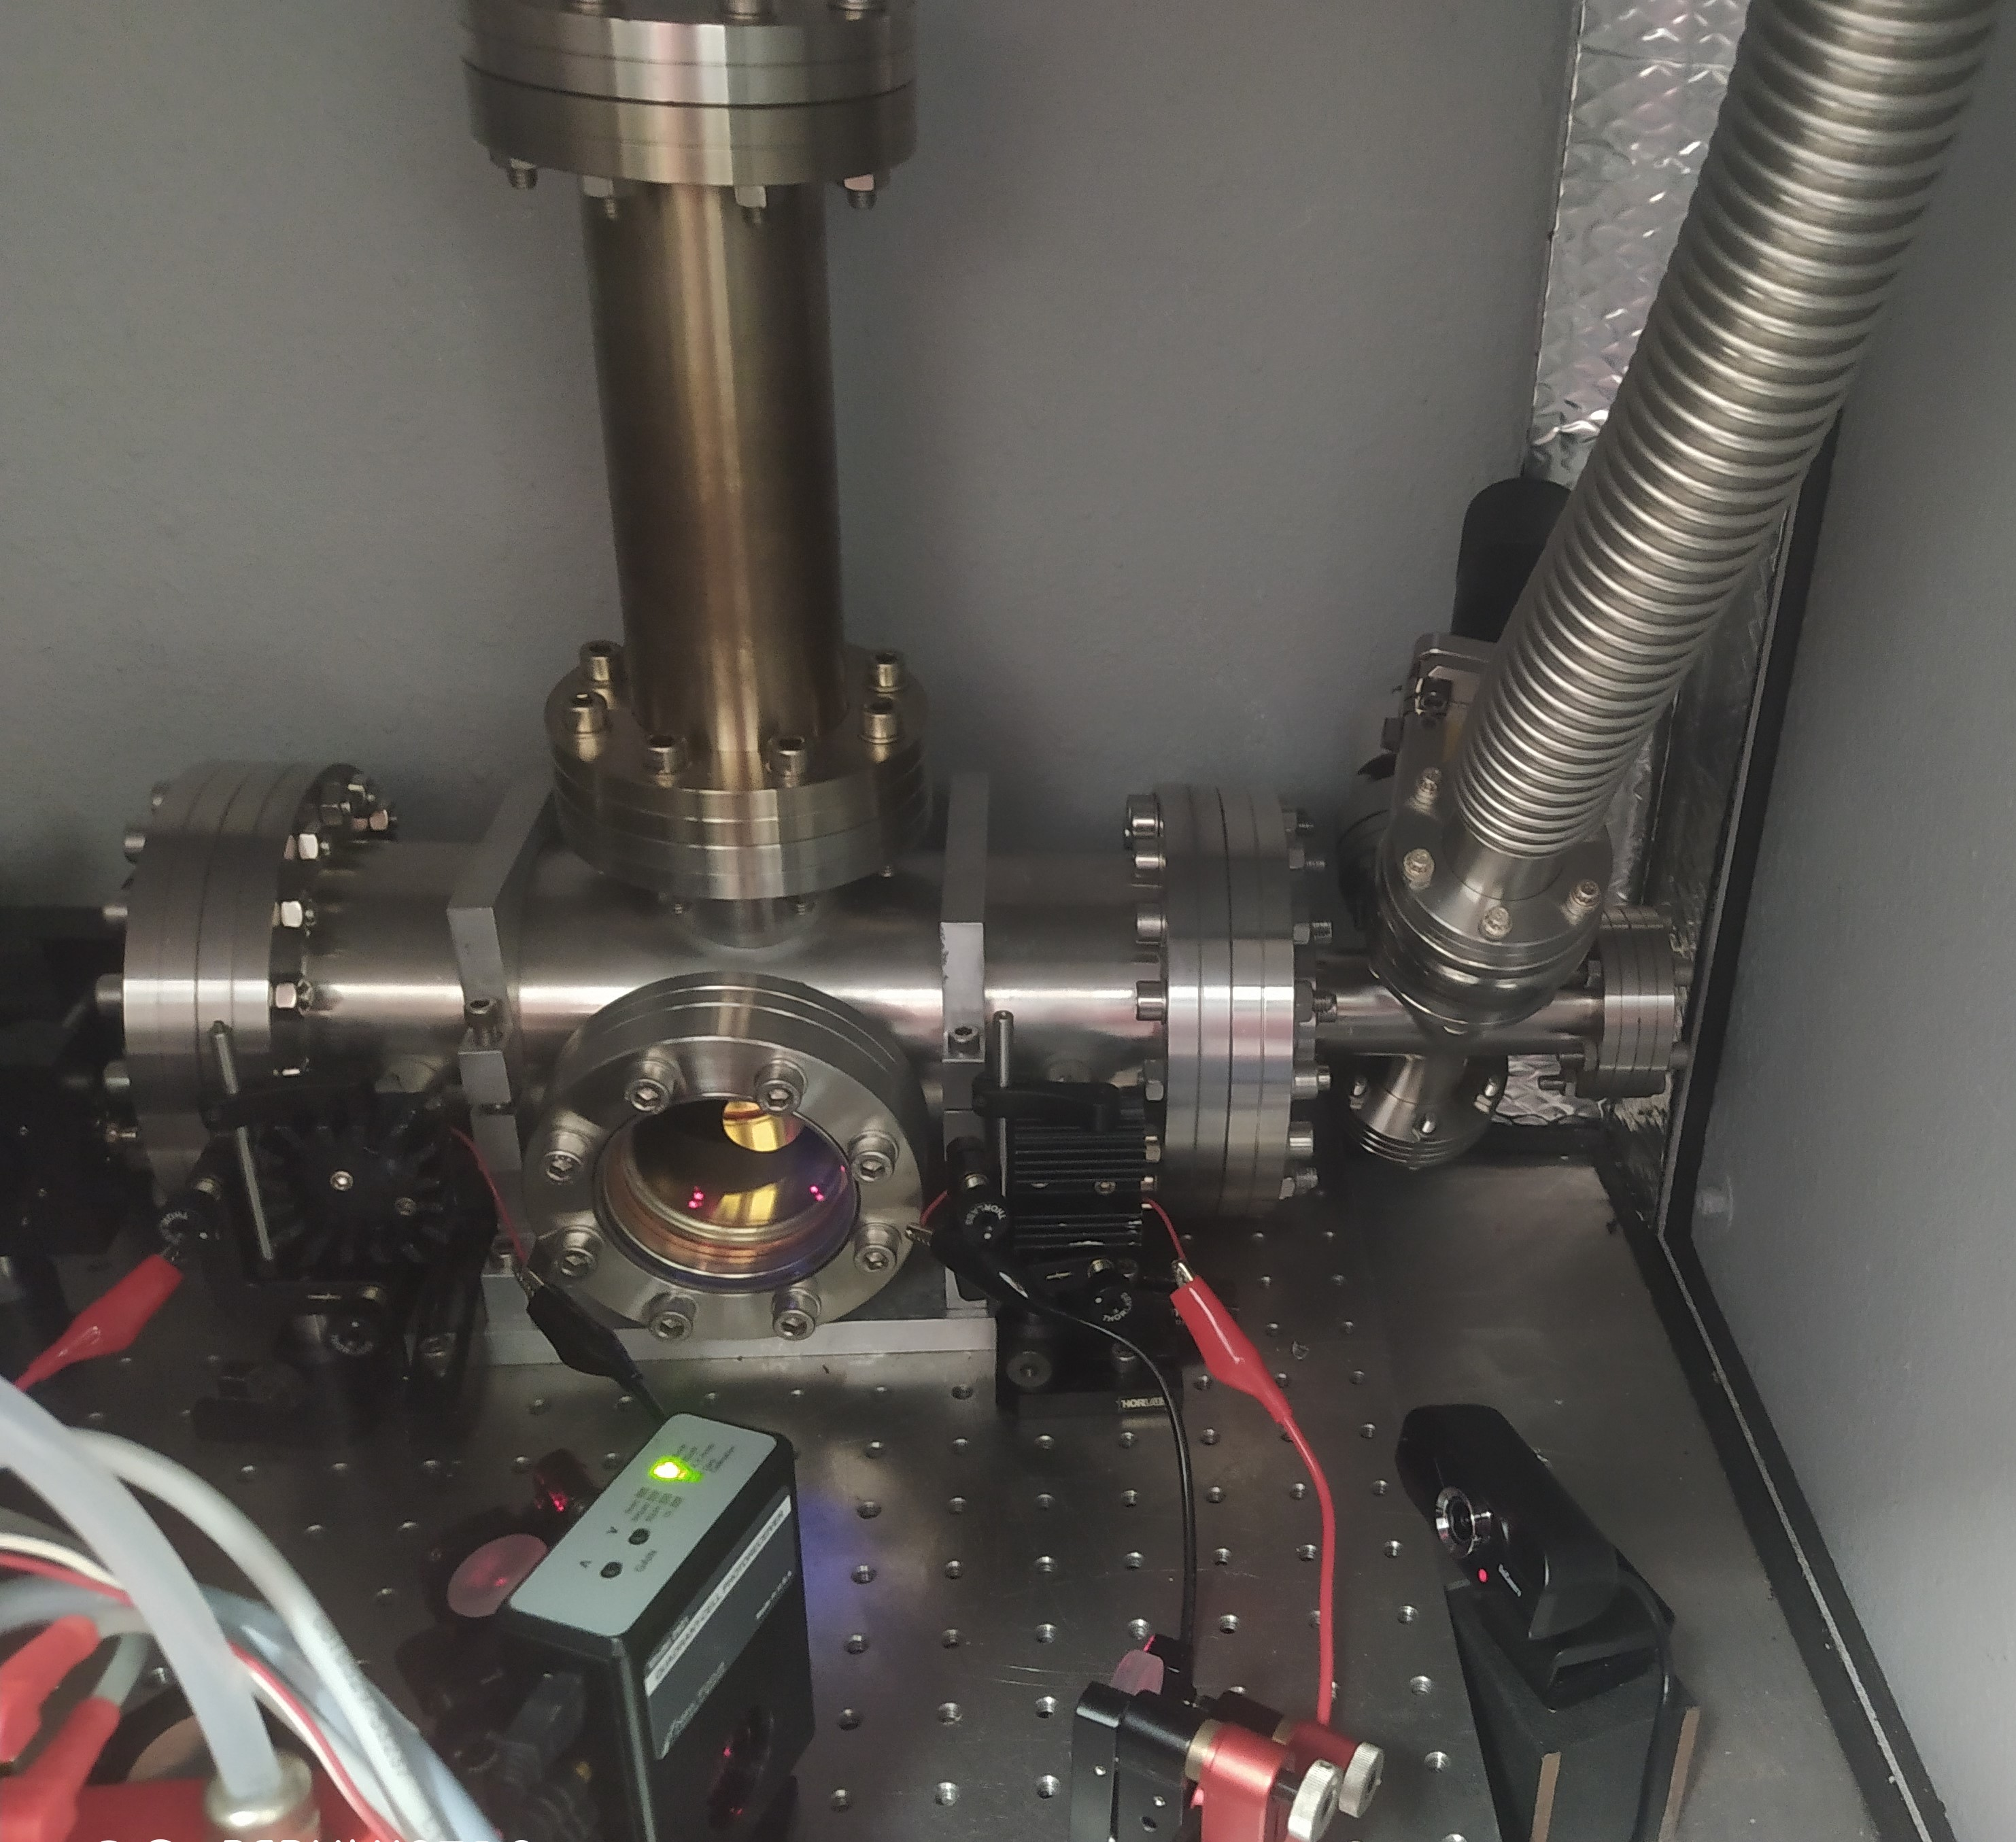
\includegraphics[scale=0.2]{\main/images/4 - methods and results/actual system_crop.jpg}}
	\caption[The measurement setup]{The measurement setup}
	\label{fig:actual system}
\end{figure}
The measurement setup inside the acoustic box after assembling is shown in fig.~\ref{fig:actual system}. Using the PID we are able to damp down the torsional pendulum oscillations, shown in fig.~\ref{fig:measured oscillation angle}. Since the damping is depended on the amplitude size (eq.~\ref{eqn:pid damping coefficient}), the damping accelerates as the amplitude gets smaller. The damping time from amplitude of $\theta_{max} = 60 [\mu rad] $ to $\theta_{max} = 10[\mu rad] $ is $3700[s]$, compares to a damping time of $250[s]$ to reach an amplitude of $\theta_{max} = 0.2[\mu rad]$.

\begin{figure}[htbp]
	\centering
	\fbox{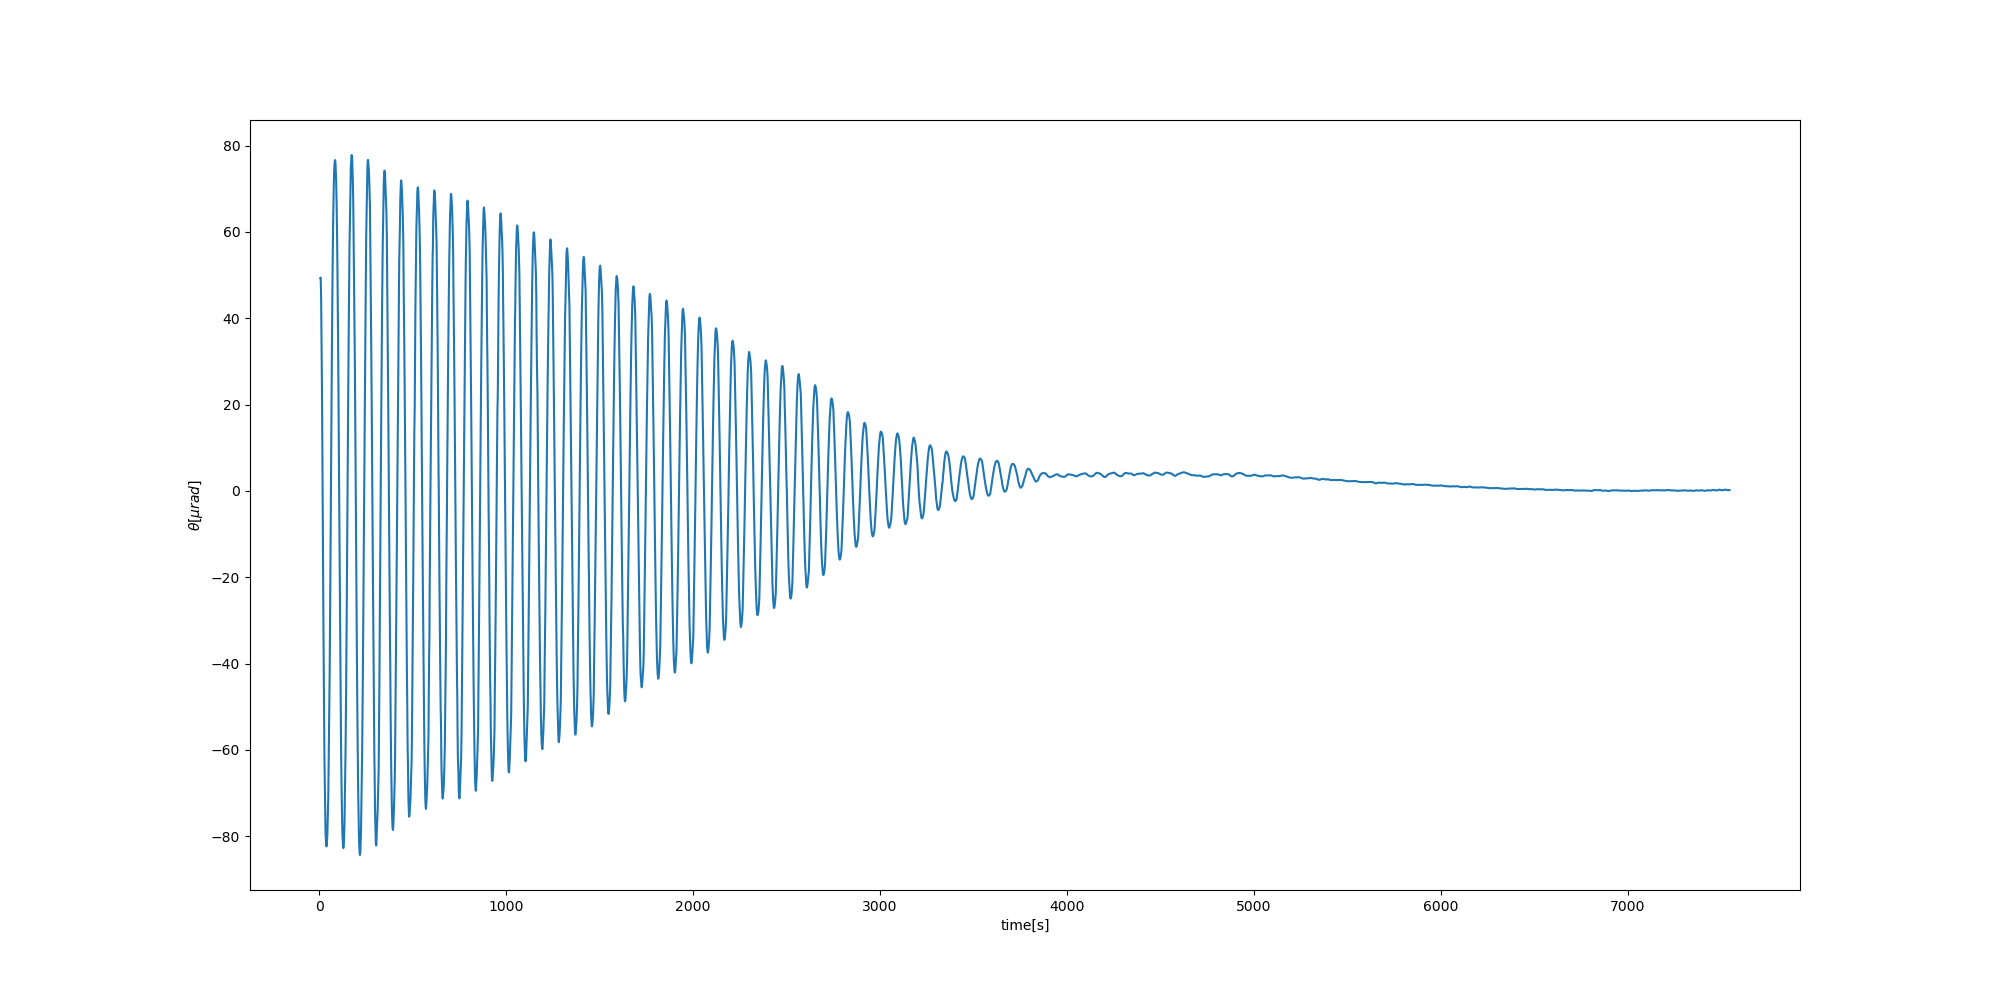
\includegraphics[scale=0.17]{\main/images/4 - methods and results/measured oscillation angle.png}}
	\caption[The damped torsional pendulum oscillations]{The damped torsional pendulum oscillations}
	\label{fig:measured oscillation angle}
\end{figure}
\par\noindent
Shown in fig.~\ref{fig:measured oscillation angle 1} are the torsional pendulum damped oscillations. The PID is able to damp up to amplitude of $\theta_{max}^{PID}= 0.05[\mu rad]$ with an average amplitude kept by the PID over time of $\overline{\theta_{max}^{PID}} = 0.2 [\mu rad]$. Having a constant amplitude over time, allows to integrate over the results. The damping is limited due to the PID tourqe power, noise, phase delay (from filtering the bouncing mode of the torsional pendulum), and not having the right PID tuning parameters (which are achieved experimentally).
\begin{figure}[htbp]
	\centering
	\fbox{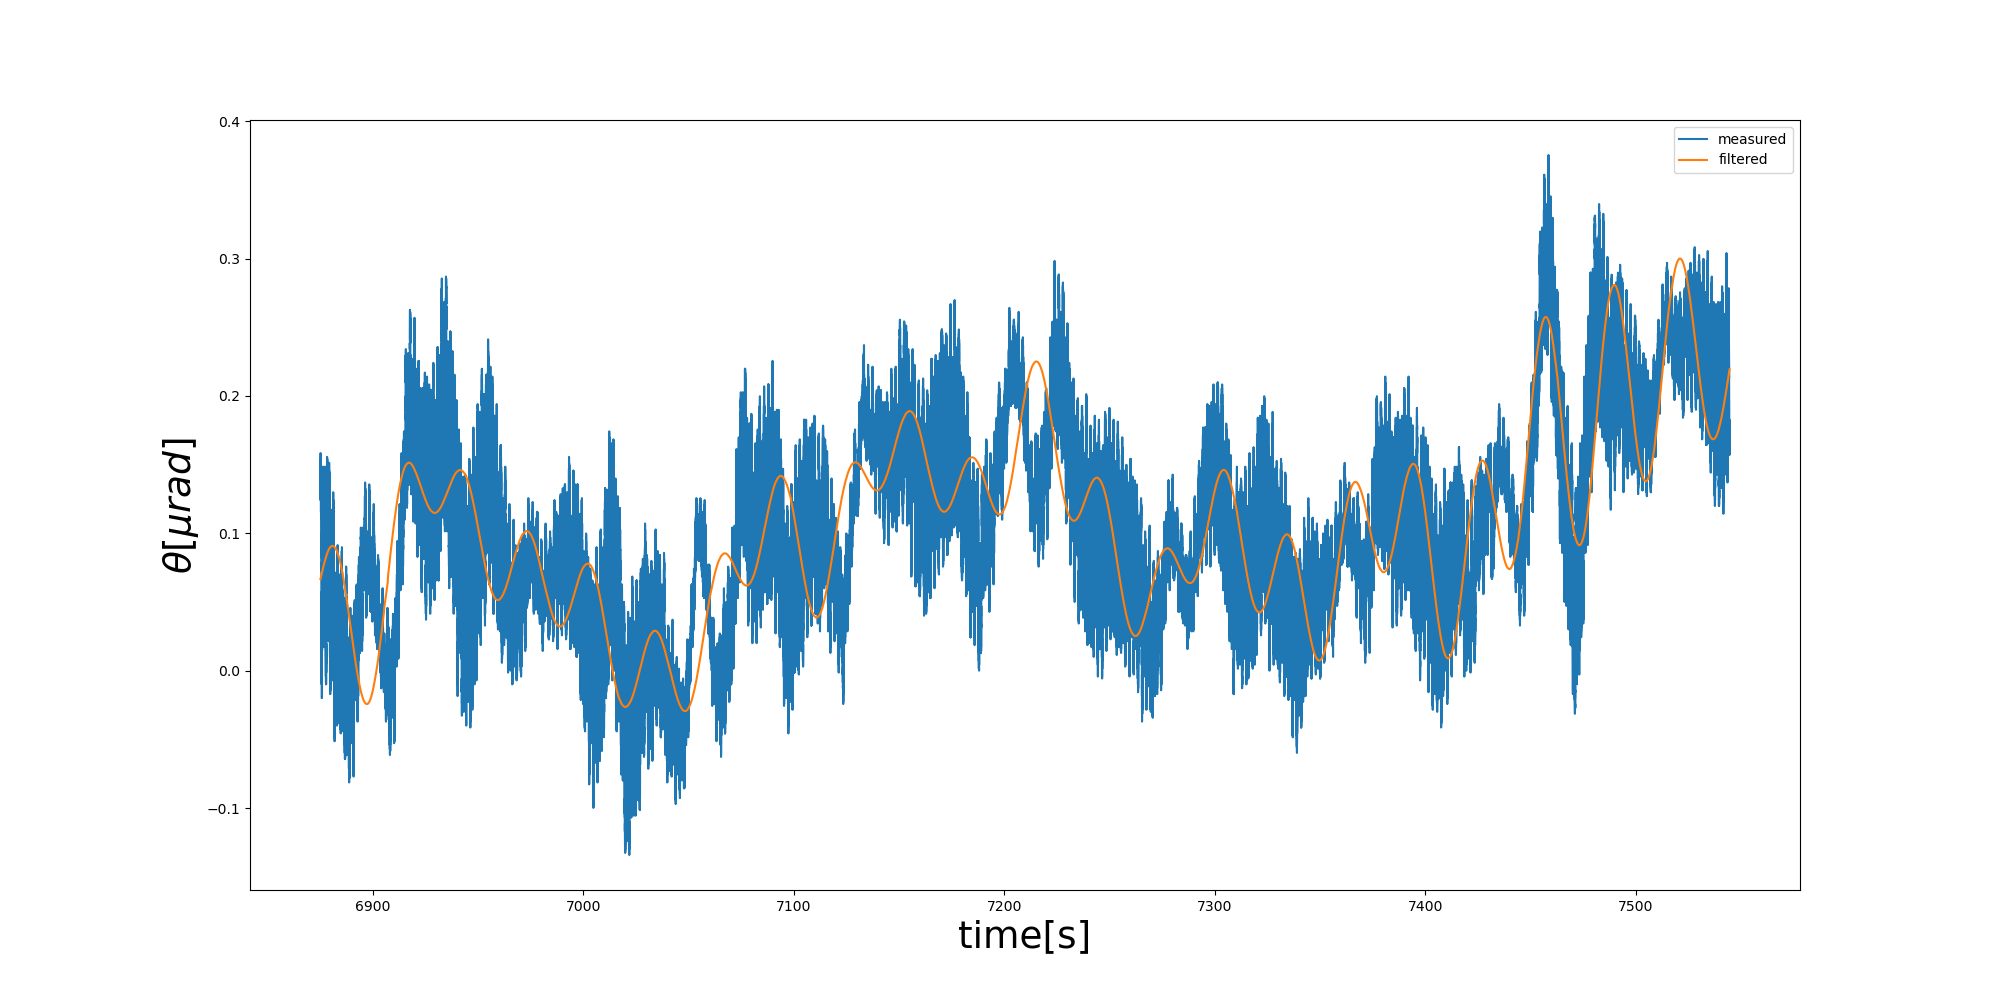
\includegraphics[scale=0.17]{\main/images/4 - methods and results/measured oscillation angle1.png}}
	\caption[The torsional pendulum minimal damped angle]{The torsional pendulum minimal damped angle}
	\label{fig:measured oscillation angle 1}
\end{figure}

\subsection{Quality factor (Q)}
Quality factor ($Q$) is a dimensionless parameter describing how underdamped is the oscillator, it is defined as the ratio of the maximum energy $U$ stored in the oscillator to the energy dissipated per cycle of oscillation. When $Q > 0.5$ the oscillator is underdamped, $Q = 0.5$ critically damped and over damped when $Q < 0.5$.
\par\noindent
Assuming negligible air friction, the energy lost in one cycle is the work done at the cycle $W_T$, which is the difference between the PID work and the environment coupled noise power $p$. Assuming the coupled noise power at the cycle is independent of time (mainly temperature and pressure dependent), the torsional pendulum Quality factor $Q$ is given by:
\begin{equation}
Q = 2\pi\cdot \frac{U}{W_T}=  \frac{2\pi\cdot(\frac{\kappa\cdot\theta(t)^2}{2}+\frac{I\cdot\dot{\theta}(t)^2}{2})}{\int_0^T[\tau_{PID}(t)\cdot\dot{\theta}(t) - p]dt} =  \frac{\pi\cdot(\kappa\theta_{max}^2cos^2(\omega\cdot 0)+I\omega^2\theta_{max}^2sin^2(\omega\cdot 0) }{\int_0^T\frac{\tau_{max} }{\theta_{max}} \frac{ T}{2\pi}(\frac{2\pi}{T}\theta_{max})^2 sin(\frac{2\pi}{T}t)dt-p\int_0^T dt }
\label{eqn:Q}
\end{equation}
\begin{equation}
Q(\theta_{max},p)  =  \frac{\pi\kappa\theta_{max}^2}{T\cdot(\frac{\theta_{max}\pi\tau_{max}}{T} -p)} \stackrel{p= 0}{=} \frac{\kappa\theta_{max}}{\tau_{max}}
\label{eqn:Q}
\end{equation}
The damping would have a non negligible effect on the motion when the oscillator is not highly underdamped $Q < 1$. It can be seen from eq.~\ref{eqn:Q} that $Q$ is highly depended on the amplitude size, even when assuming no environmental noises ($p=0$), the amplitudes with which the damping affects the motion are:  
\begin{equation}
\theta_{max}(Q<1,p=0) < \frac{\tau_{max}}{\kappa} \approx \frac{3.4\cdot 10^{-10}}{2.7\cdot 10^{-6}} \approx 125 [\mu rad]
\label{eqn:low Q}
\end{equation}

It can be seen from eq.~\ref{eqn:Q} that when $Q<0$ the coupled noise power is larger than the work done by the PID, causing the oscillator to be driven. When assuming the noise power is the limiting factor of the damping, one can estimate the coupled noise power from the measured damped amplitude of the torsional pendulum $p \rightarrow \frac{ \theta_{max}^{PID}\pi\tau_{max}}{T}$, resulting with $Q(\theta_{max}^{PID},p)	\rightarrow 0$. Fig.~\ref{fig:Q factor} is a plot of $Q(\theta_{max},p)$, with noise powers  of $p= 8\cdot 10^{-18} - 1\cdot 10^{-18} [W]$, which result  with $Q(\theta_{max}^{PID} = 0.2 [\mu rad],p = 8\cdot 10^{-18}) 	\rightarrow 0$ at the actual measured damped amplitudes $\theta_{max}^{PID}= 0.2 [\mu rad] -0.05 [\mu rad]$, resulting with coupled noise power.

\begin{figure}[htbp]
	\centering
	\fbox{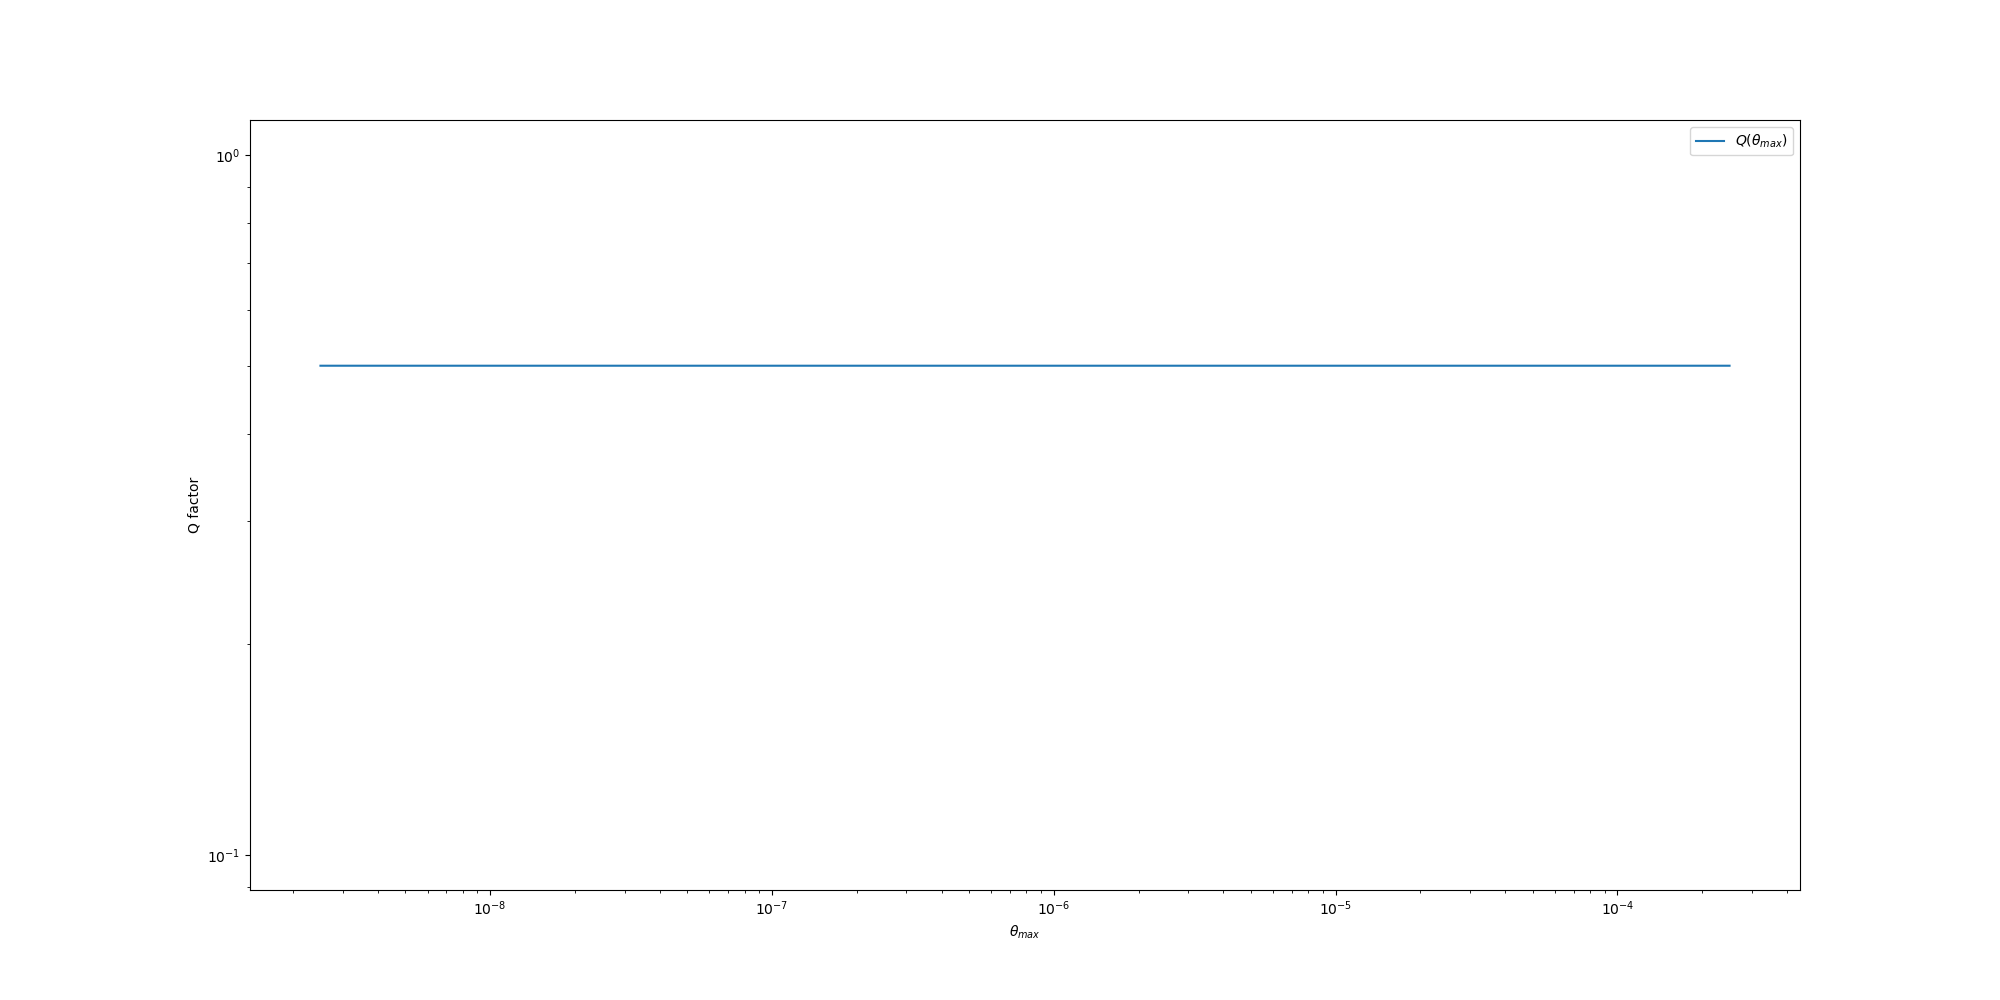
\includegraphics[scale=0.11]{\main/images/4 - methods and results/Q factor.png}}
	\caption[The torsional pendulum Q factor]{The torsional pendulum Q factor}
	\label{fig:Q factor}
\end{figure} 

\subsection{Brownian motion}
Due to Brownian motion, we estimate $n_p= \frac{N}{V}v A$ gas particles collisions per second into the cross section of the torsional pendulum. Each gas particle is with mass $m_0 = \frac{M}{N_A}$ and mean velosity of the gas flow $v$ (eq.~\ref{eqn:flow velocity}). Assuming all collisions are elastic, the particles exchanges mean momentum of $k=2m_0v$, resulting with force $F = n_p\cdot k$. Due to the collisions the torsional pendulum velosity is $ u = n_p\frac{k}{m_1}$, resulting with power given by:
\begin{equation}
p = F\cdot u =  n_p k \cdot n_p\frac{k}{m_1} =\frac{4}{m_1}(\frac{N}{V}v A)^2m_0^2v^2=\frac{4A^2}{m_1}(\frac{P}{k_B T})^2(\frac{M}{N_A})^2 (\frac{3 k_B N_A T}{M})^2 =\frac{36A^2P^2}{m_1} 
\label{eqn:Brownian power}
\end{equation}
\subsection{Noise power}
As shown previously, there are multiple noise sources at the environment. Assuming gas and environment temperature of $T = 298K$ and torsional pendulum temperature $T_0 = 0K$ (maximal noise power), the noise power is given by:
\begin{multicols}{2}
\raggedcolumns
\begin{easylist}
& Thermal flow (eq.~\ref{eqn:heat conduction});
&& $p=0.083[W]$.
& Black body radiation (eq.~\ref{eqn: Stefan–Boltzmann power}, \cite{WOODS201444});
&& $p=0.121[W]$.
\end{easylist}
\columnbreak
\begin{easylist}
& Brownian motion (eq.~\ref{eqn:Brownian power});
&& $p=6.2\cdot 10^{-6}[W]$.
& Acoustic waves (eq.~\ref{eqn:acoustic power});
&& $p=1.1\cdot 10^{-28}[W]$.
\end{easylist}
\end{multicols}
\par\noindent
Even at room temperature the power from Brownian motion is much larger than estimated previously ($p= 8\cdot 10^{-18} - 1\cdot 10^{-18} [W]$). Which leads to estimate the effective driving noise only as the effective collision power. Which means thermal flow does not couple noise into the system, and the noise coupled by the black body radiation is the radiation force caused by the photons colliding into the torsional pendulum. 
\subsection{Random motion}
Due to random motion, $n_p$ particles collide per second into cross section $A$ of mass $m_1$. Random motion can be modelled as a Poisson process, and the effective collision rate is the square root of the number of events $n_{col} = \sqrt{n_p}$. Each particle exchanges momentum $k$ with with $m_1$, resulting with force $F = n_{col}\cdot k$. Due to the collisions the velosity of $m_1$ is $ u = n_{col}\frac{k}{m_1}$. The collisions result with power given by:
\begin{equation}
p = F\cdot u =  n_{col}k \cdot n_{col}\frac{k}{m_1} =  n_p\frac{ k^2}{m_1}
\label{eqn:net power}
\end{equation}
The Brownian motion collision power is given in eq.~\ref{eqn:Brownian power}. Thus, the effective Brownian power $p_{eff}$, is given by:
\begin{equation}
p_{eff} =  n_p\frac{ k^2}{m_1} = \frac{p}{n_p} = \frac{\frac{36A^2P^2}{m_1}}{\frac{N}{V}v A} = \frac{12AP}{m_1}\sqrt{\frac{3 k_B T M}{ N_A }}
\label{eqn:Brownian net power}
\end{equation}
Due to environmental black body radiation (see eq.~\ref{eqn: Stefan–Boltzmann power}) there are photons colliding into $A$. It can be shown that the mean energy of a black body photon is $E\approx 2.7k_B T$, resulting with $n_p = \frac{j}{E}A$ photon collisions. The incident photons composed of reflected flux $j_{ref}=(1-\epsilon)\sigma T^4$ with elastic collision and momentum of $k_{ref} = \frac{2E}{c} $, and absorbed flux $j_{ab}=\epsilon\sigma T^4$ with momentum of $k_{ab} = \frac{E}{c}$. Thus, the effective black body radiation power $p_{eff}$, is given by:
\begin{equation}
p_{eff} =  n_p\frac{ k^2}{m_1} = \frac{j_{ref}}{E}A\cdot\frac{ (\frac{2E}{c})^2}{m_1} +\frac{j_{ab}}{E}A\cdot\frac{ (\frac{E}{c})^2}{m_1} = \frac{  2.7 A k_B T }{ c^2 m_1} (4j_{ref}+j_{ab}) =\frac{2.7A k_B}{ c^2 m_1} (4-3\epsilon)\sigma T^5 
\label{eqn:photon collision power}
\end{equation}
The effective noise power composed by Brownian motion, acoustic waves and black body radiation both is pressure dependent and  environment temperature dependent (room temperature $T$). The effective noise power is given by:
\begin{equation}
p_{eff}  \approx A (10^{-22}P^2+ 3.8\cdot 10^{-21}P +1.1\cdot 10^{-45}T^5) \approx 4.4\cdot 10^{-25}  [W]
\label{eqn:net power}
\end{equation} 
\end{document}